% document class and packages
\documentclass{beamer}
\usepackage{adjustbox}
\usepackage{algorithm,algorithmic}
\usepackage{amsmath}
\usepackage{amssymb}
\usepackage{color, colortbl}
\usepackage{graphicx}
\usepackage{hyperref}
\usepackage{pgfplots}
\pgfplotsset{compat=1.14}
\usepackage{tikz}

% indent for algorithm pseudo-code
\newlength\myindent
\setlength\myindent{1em}
\newcommand\bindent{%
  \begingroup
  \setlength{\itemindent}{\myindent}
  \addtolength{\algorithmicindent}{\myindent}
}
\newcommand\eindent{\endgroup}

% new commands and operators
\newcommand\diag[1]{\operatorname{diag}\left(#1\right)}
\newcommand\abs[1]{\left|#1\right|}
\newcommand\norm[1]{\left\Vert#1\right\Vert}
\newcommand{\iu}{{i\mkern1mu}}
\newcommand\hd[2]{\operatorname{hd}(#1,#2)}
\newcommand\specR[1]{\operatorname{specR}(#1)}
\newcommand\connR[1]{\operatorname{connR}(#1)}
\newcommand\func[1]{\operatorname{function}~[#1]}

% 
\newtheorem{proposition}[theorem]{Proposition}

% remove figure caption prefix
\setbeamertemplate{caption}{\raggedright\insertcaption\par}

% hyperlinks setup
\hypersetup{colorlinks,breaklinks,
	urlcolor=[rgb]{0,0.75,1},
	linkcolor=[rgb]{0.75,0.75,0.75}}

% empty navigation symbols
\beamertemplatenavigationsymbolsempty

% remove navigation dots on miniframes
\makeatletter
\def\beamer@writeslidentry{\clearpage\beamer@notesactions}
\makeatother

% Use Theme
\usetheme{Warsaw}
\useoutertheme[footline=authortitle]{miniframes}
\useinnertheme[shadow=true]{rounded}

% Colors
\definecolor{black}{RGB}{0, 0, 0} % (primary, black)
\definecolor{lblue}{RGB}{102, 178, 255} % (secondary, light blue)
\definecolor{lgreen}{RGB}{102, 255, 178} %(tertiary, light green)
\definecolor{lsilver}{RGB}{224,224,224} % (text, light silver)
\definecolor{gray}{RGB}{128,128,128} % (graph node shade, gray)
\definecolor{white}{RGB}{255,255,255} % (graph node text, white)

% Beamer Colors
\setbeamercolor{palette primary}{bg=black,fg=lsilver}
\setbeamercolor{palette secondary}{bg=lblue,fg=lsilver}
\setbeamercolor{palette tertiary}{bg=black,fg=lsilver}
\setbeamercolor{structure}{fg=black} % itemize, enumerate, etc
\setbeamercolor{frametitle}{fg=black}

% Transparency for itemized listing
%\setbeamercovered{transparent}

% Title Page
\title{Rankability, Predictability, and Ellipses}
\author{Thomas R. Cameron}
\institute{Davidson College}
\date{June 4, 2019}

\begin{document}
% Title Frame
\begin{frame}
	\titlepage
\end{frame}

% Outline
%\AtBeginSection[]{
 %\frame<beamer>{
  %\frametitle{Outline}   
  %\tableofcontents[currentsection]
 %}
%}

%%%%%%%%%%%%%%%%%%%%%%%%%%%%%%%%%%%%%%%%%%%%%%%%%%%%%%
%								Measures of Rankability
%%%%%%%%%%%%%%%%%%%%%%%%%%%%%%%%%%%%%%%%%%%%%%%%%%%%%%
\section{Measures of Rankability}

\begin{frame}{Spectral Rankability}
\begin{algorithm}[H]
\caption{Spectral Rankability of Graph Data $\Gamma$.}
\begin{algorithmic}
\STATE{$\func{r} = \specR{\Gamma}:$}
\bindent
\STATE{$n\gets$ the number of vertices in $\Gamma$}
\STATE{$D\gets$ the degree matrix of $\Gamma$}
\STATE{$L\gets$ graph Laplacian of $\Gamma$}
\STATE{$s=\diag{n-1,n-2,\ldots,0}$}
\STATE{$r=\frac{\hd{D}{S}+\hd{L}{S}}{2(n-1)}$}
\RETURN
\eindent
\end{algorithmic}
\end{algorithm}
\end{frame}

\begin{frame}{Connectivity Rankability}
\begin{algorithm}[H]
\caption{Connectivity Rankability of Graph Data $\Gamma$.}
\begin{algorithmic}
\STATE{$\func{r} = \connR{\Gamma}:$}
\bindent
\STATE{$n\gets$ the number of vertices in $\Gamma$}
\STATE{$L\gets$ graph Laplacian of $\Gamma$}
\STATE{$\alpha = \min_{x\in S}x^{T}Lx$, where $S=\{x\in\mathbb{R}^{n}\colon x\perp e, \norm{x}=1\}$}
\STATE{$\beta = \max_{x\in S}x^{T}Lx$, where $S=\{x\in\mathbb{R}^{n}\colon x\perp e, \norm{x}=1\}$}
\STATE{$\tilde{\alpha}\gets$ related quantity for perfect dominance graph}
\STATE{$\tilde{\beta}\gets$ related quantity for perfect dominance graph}
\STATE{$r=\frac{\abs{\alpha-\tilde{\alpha}} + \abs{\beta-\tilde{\beta}}}{2n}$}
\RETURN
\eindent
\end{algorithmic}
\end{algorithm}
\end{frame}

%%%%%%%%%%%%%%%%%%%%%%%%%%%%%%%%%%%%%%%%%%%%%%%%%%%%%%
%								Big East Football
%%%%%%%%%%%%%%%%%%%%%%%%%%%%%%%%%%%%%%%%%%%%%%%%%%%%%%
\section{Big East Football}

\begin{frame}{Results}
\begin{minipage}{0.45\textwidth}
\centering
\resizebox{\textwidth}{!}{%
\begin{tabular}{|| c | c | c | c | c | c || }
\hline
Year & specR & connR & Massey & Colley & Cycles \\
\hline
1995 & 0.143 & 0.043 & 0.893 & 0.926 & 7 \\
1996 & 0.143 & 0.043 & 0.857 & 0.963 & 1 \\
1997 & 0.185 & 0.069 & 0.679 & 0.714 & 62 \\
1998 & 0.183 & 0.062 & 0.750 & 0.889 & 30 \\
1999 & 0.143 & 0.058 & 0.821 & 0.889 & 23 \\
2000 & 0.143 & 0.002 & 0.929 & 0.929 & 3 \\
2001 & 0.143 & 0.001 & 0.857 & 1.000 & 1 \\
2002 & 0.143 & 0.005 & 0.893 & 0.963 & 3 \\
2003 & 0.143 & 0.049 & 0.786 & 0.885 & 18 \\
2004 & 0.339 & 0.168 & 0.762 & 0.778 & 48 \\
2005 & 0.162 & 0.013 & 0.821 & 0.885 & 16 \\
2006 & 0.195 & 0.100 & 0.750 & 0.808 & 45 \\
2007 & 0.316 & 0.169 & 0.643 & 0.654 & 205 \\
2008 & 0.195 & 0.099 & 0.714 & 0.852 & 43 \\
2009 & 0.143 & 0.049 & 0.786 & 0.857 & 26 \\
2010 & 0.292 & 0.166 & 0.750 & 0.741 & 174 \\
2011 & 0.286 & 0.149 & 0.643 & 0.808 & 125 \\
2012 & 0.286 & 0.163 & 0.643 & 0.769 & 111 \\
\hline
\end{tabular}%
}
\end{minipage}\hfill
\begin{minipage}{0.45\textwidth}
\centering
\resizebox{\textwidth}{!}{%
\begin{tabular}{|| c | c | c | c ||}
\hline
& Massey & Colley & Cycles \\
\hline
specR & -0.719 & -0.785 & 0.826 \\
connR & -0.802 & -0.829 & 0.843 \\
\hline
\end{tabular}%
}
\end{minipage}
\end{frame}

%%%%%%%%%%%%%%%%%%%%%%%%%%%%%%%%%%%%%%%%%%%%%%%%%%%%%%
%								MBB Southern Conference
%%%%%%%%%%%%%%%%%%%%%%%%%%%%%%%%%%%%%%%%%%%%%%%%%%%%%%
\section{MBB Southern Conference}

\begin{frame}{Results}
\begin{minipage}{0.45\textwidth}
\centering
\resizebox{\textwidth}{!}{%
\begin{tabular}{|| c | c | c | c | c || }
\hline
Year & specR & connR & Massey & Colley \\
\hline
2002 & 0.294 & 0.174 & 0.579 & 0.654 \\
2003 & 0.227 & 0.119 & 0.710 & 0.710 \\
2004 & 0.136 & 0.088 & 0.738 & 0.785 \\
2005 & 0.147 & 0.083 & 0.729 & 0.738 \\
2006 & 0.119 & 0.060 & 0.711 & 0.722 \\
2007 & 0.155 & 0.108 & 0.771 & 0.780 \\
2008 & 0.200 & 0.058 & 0.775 & 0.775 \\
2009 & 0.227 & 0.112 & 0.756 & 0.740 \\
2010 & 0.227 & 0.147 & 0.697 & 0.706 \\
2011 & 0.094 & 0.060 & 0.748 & 0.782 \\
2012 & 0.227 & 0.130 & 0.664 & 0.664 \\
2013 & 0.273 & 0.152 & 0.790 & 0.756 \\
2014 & 0.173 & 0.100 & 0.745 & 0.776 \\
2015 & 0.340 & 0.217 & 0.720 & 0.700 \\
\hline
\end{tabular}%
}
\end{minipage}\hfill
\begin{minipage}{0.45\textwidth}
\centering
\resizebox{\textwidth}{!}{%
\begin{tabular}{|| c | c | c ||}
\hline
& Massey & Colley \\
\hline
specR & -0.339 & -0.615 \\
connR & -0.408 & -0.615 \\
\hline
\end{tabular}%
}
\end{minipage}
\end{frame}

%%%%%%%%%%%%%%%%%%%%%%%%%%%%%%%%%%%%%%%%%%%%%%%%%%%%%%
%								Ellipses
%%%%%%%%%%%%%%%%%%%%%%%%%%%%%%%%%%%%%%%%%%%%%%%%%%%%%%
\section{Ellipses}

\begin{frame}{Numerical Range}
The algebraic connectivity is the following minimization problem:
\[
\alpha = \min_{\norm{x}=1}Re(x^{*}Q^{T}LQx).
\]
\vfill
The numerical range is defined by
\[
W(Q^{T}LQ) = \left\{x^{*}Q^{T}LQx,~\norm{x}=1\right\}
\]
\end{frame}

\begin{frame}{Conjecture}
The numerical range associated with the perfect dominance graph is an ellipse!
\vfill
\centering
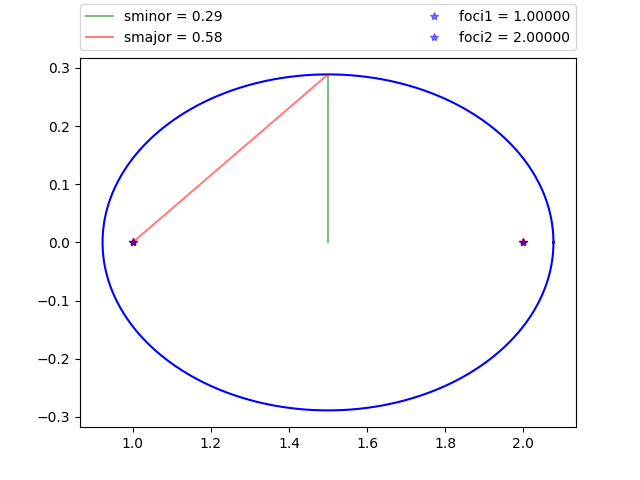
\includegraphics[scale=0.5]{figures/nr_dom1}
\end{frame}

\begin{frame}{Unique Characterization?}
The numerical range associated with a cycle is a polygon:
\vfill
\centering
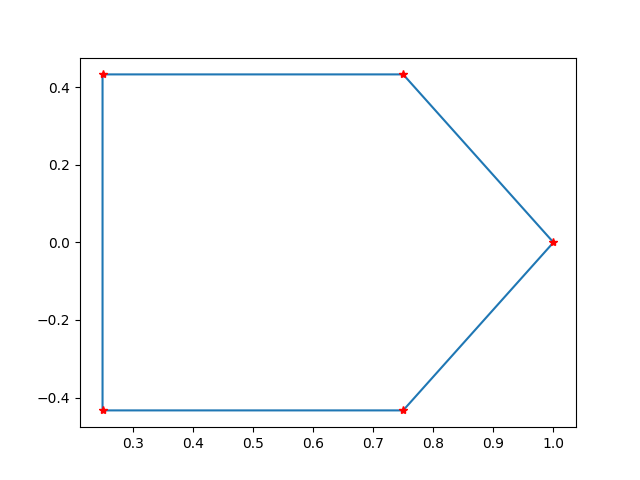
\includegraphics[scale=0.5]{figures/nr_cycle1}
\end{frame}

\end{document}